\section{How?}


\begin{frame}{The Master Plan}
  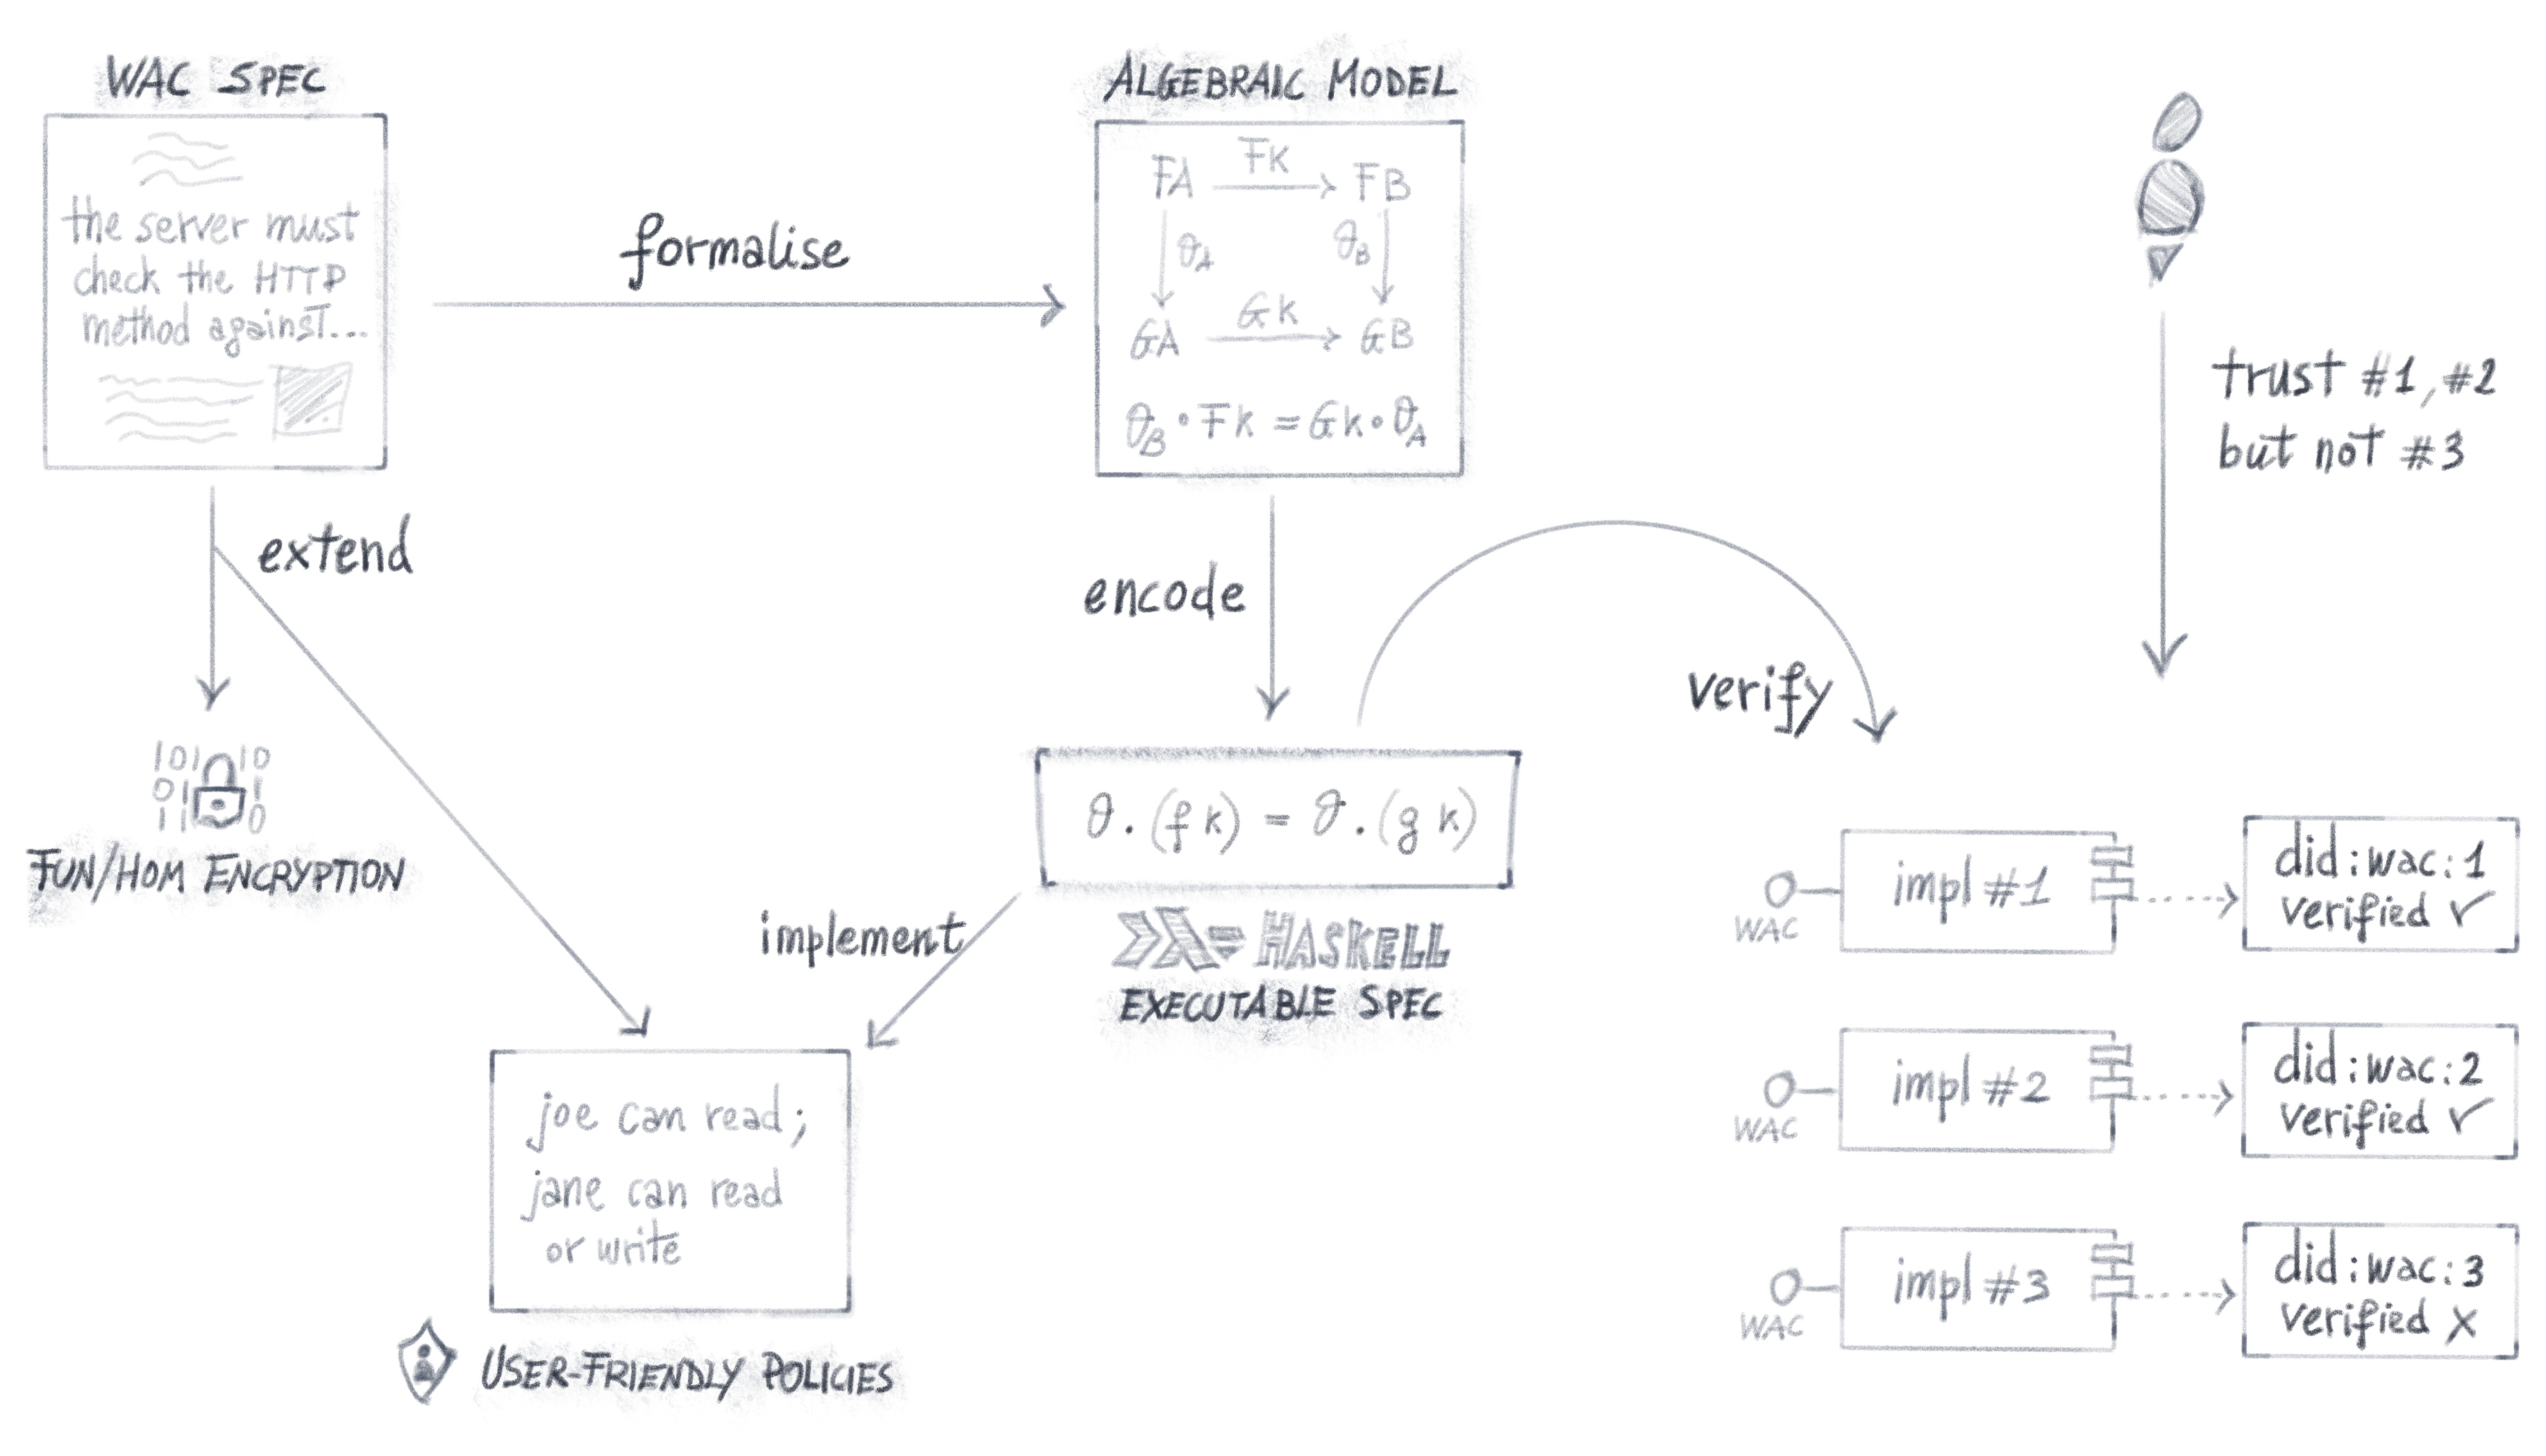
\includegraphics[height=0.65\paperheight]{./media/implementation-plan.png}
\end{frame}


\begin{frame}{Proof of Concept}

Whack WAC is open-source
\begin{itemize}
  \item \href{https://github.com/c0c0n3/whack-wac}{https://github.com/c0c0n3/whack-wac}
  \item Initial algebraic model
  \item Trivial Haskell executable spec
  \item Simple Haskell policy EDSL
\end{itemize}

\end{frame}


\begin{frame}{Formal Methods Teaser}

Approach: Adopt mathematical techniques to produce software users
can trust to be correct.

\bigskip

Hard: How to get from plain English to equations?

\bigskip

Here's a trivial example to illustrate the approach.

\end{frame}


\begin{frame}{Formal Methods Teaser}

Alice runs her business from home.

She's got a nice garden where she receives customers.

She's hired a new butler, Alfie.

Alice instructs Alfie: \emph{"Usher customers to the garden."}

\end{frame}


\begin{frame}{Formal Methods Teaser}
  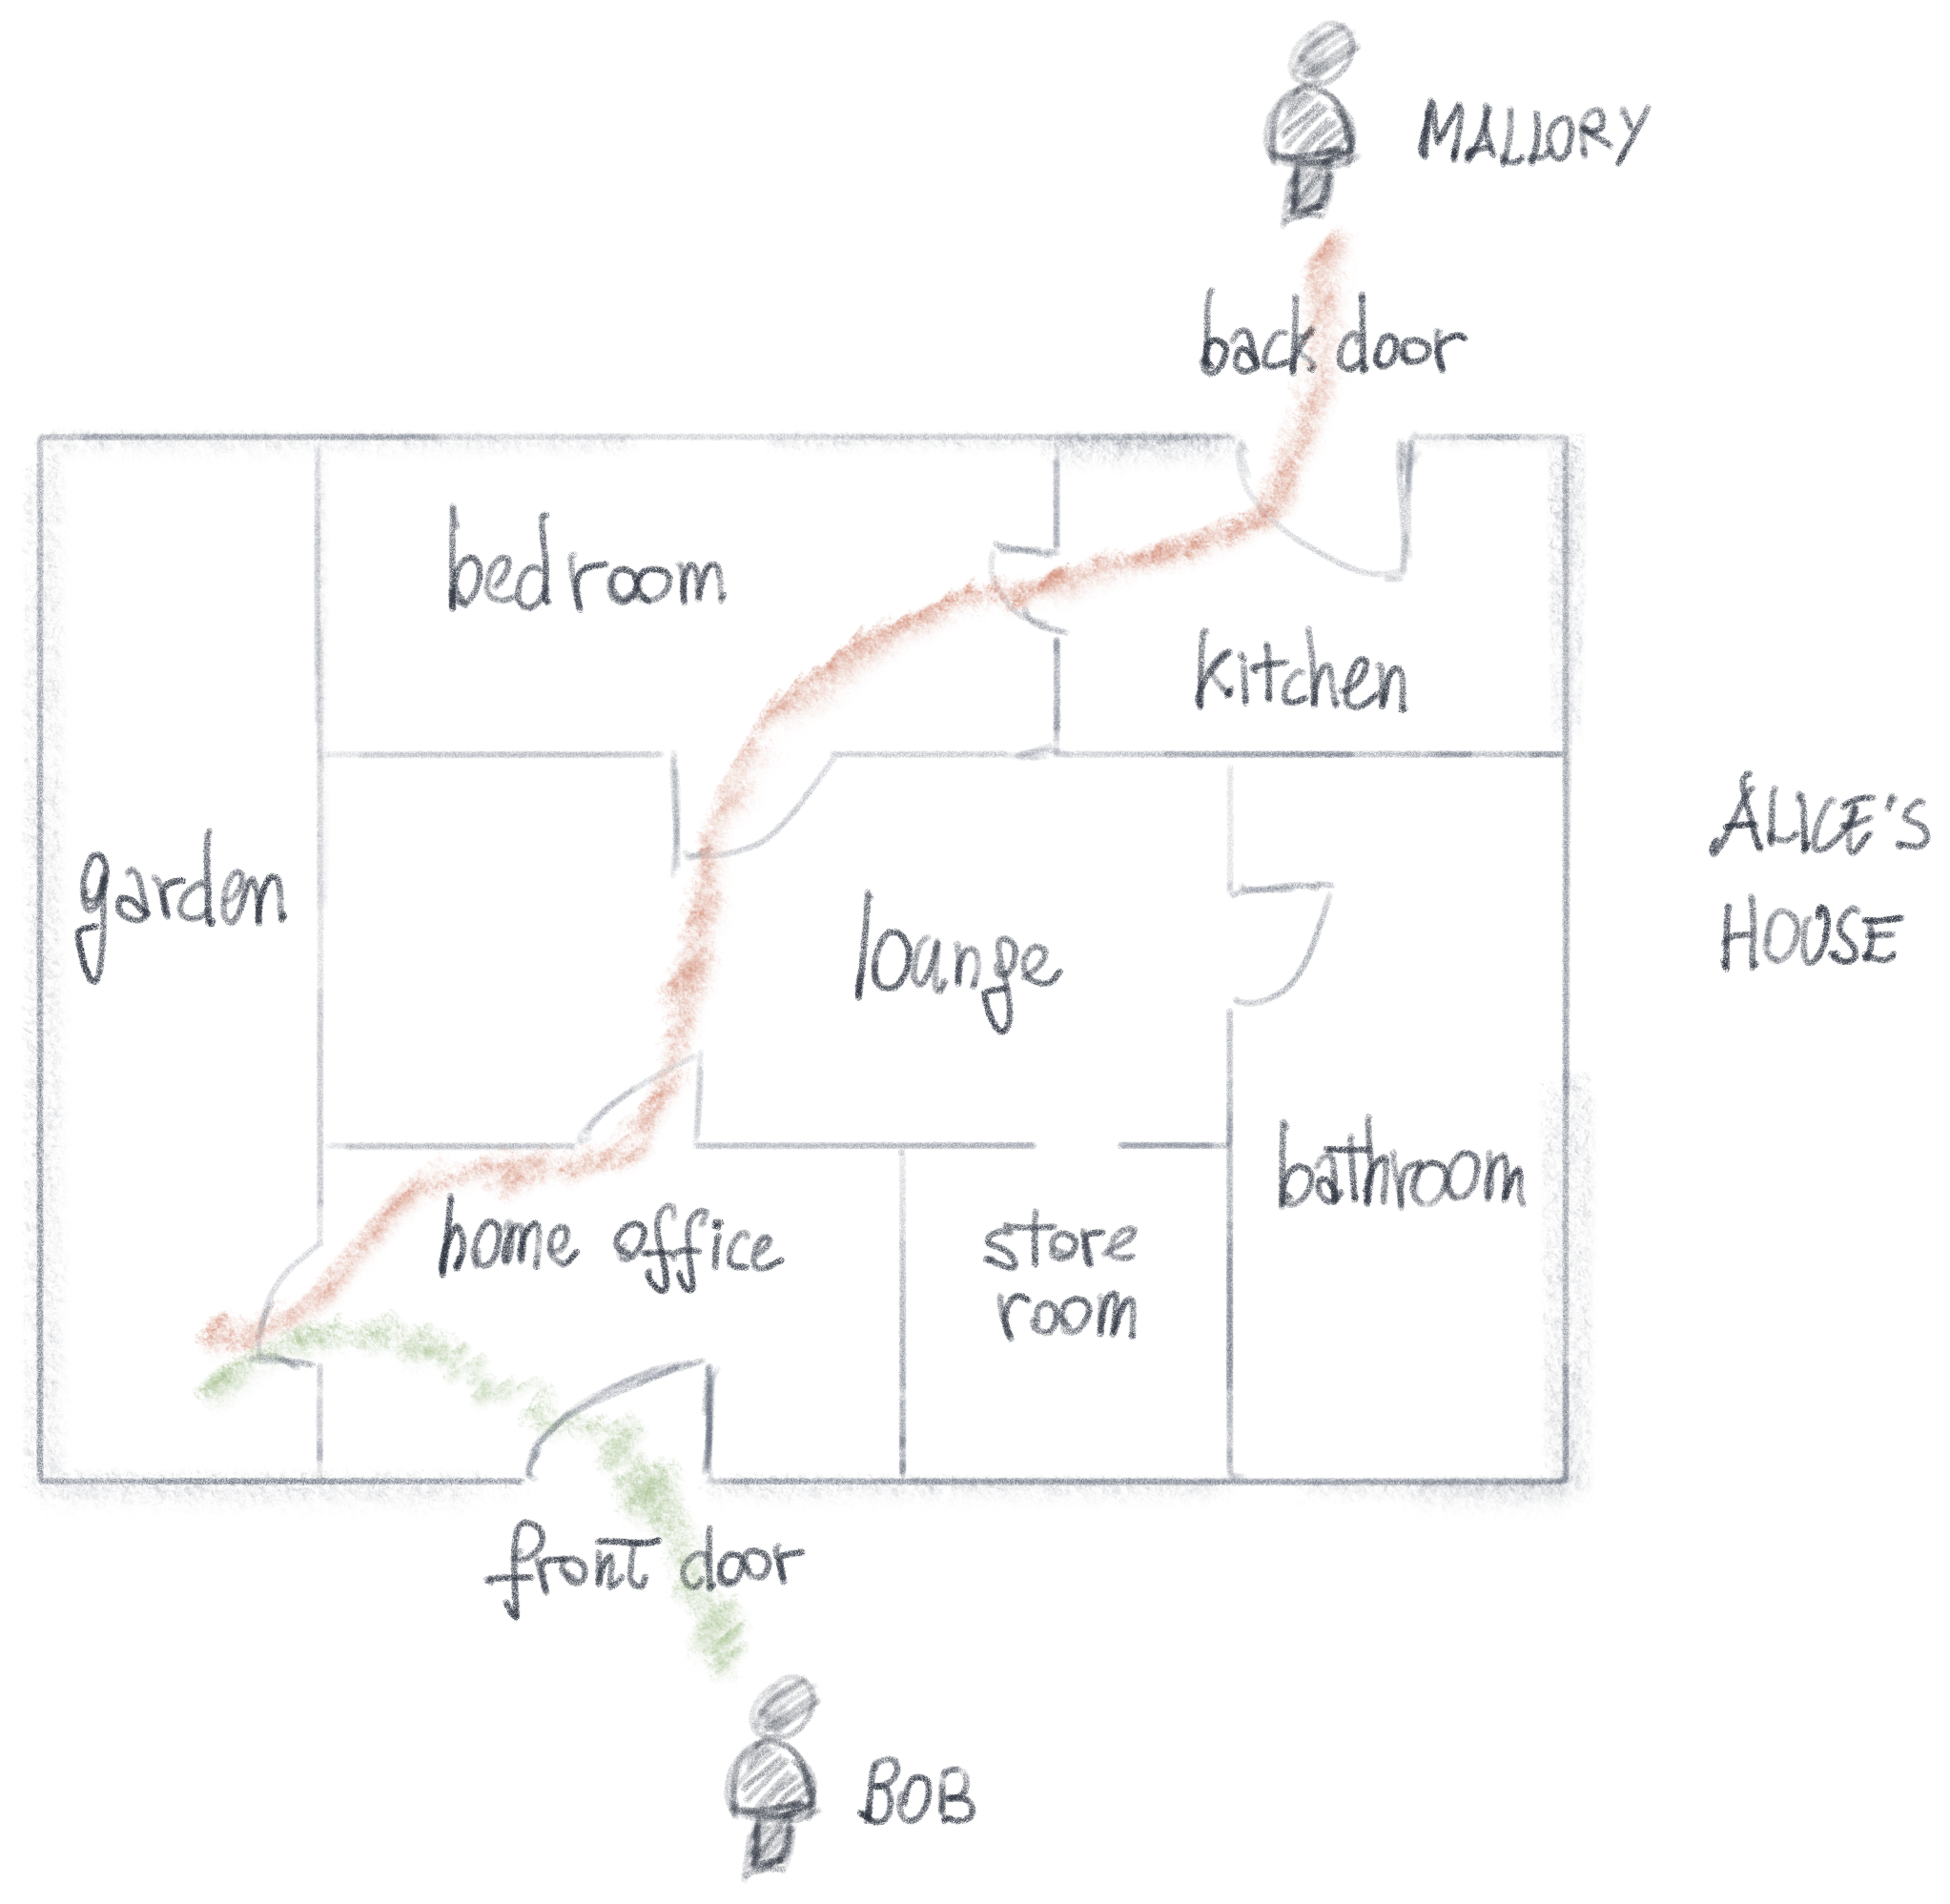
\includegraphics[height=0.8\paperheight]{./media/ambiguous-spec_trivial-example.png}
\end{frame}


\begin{frame}{Formal Methods Teaser}
  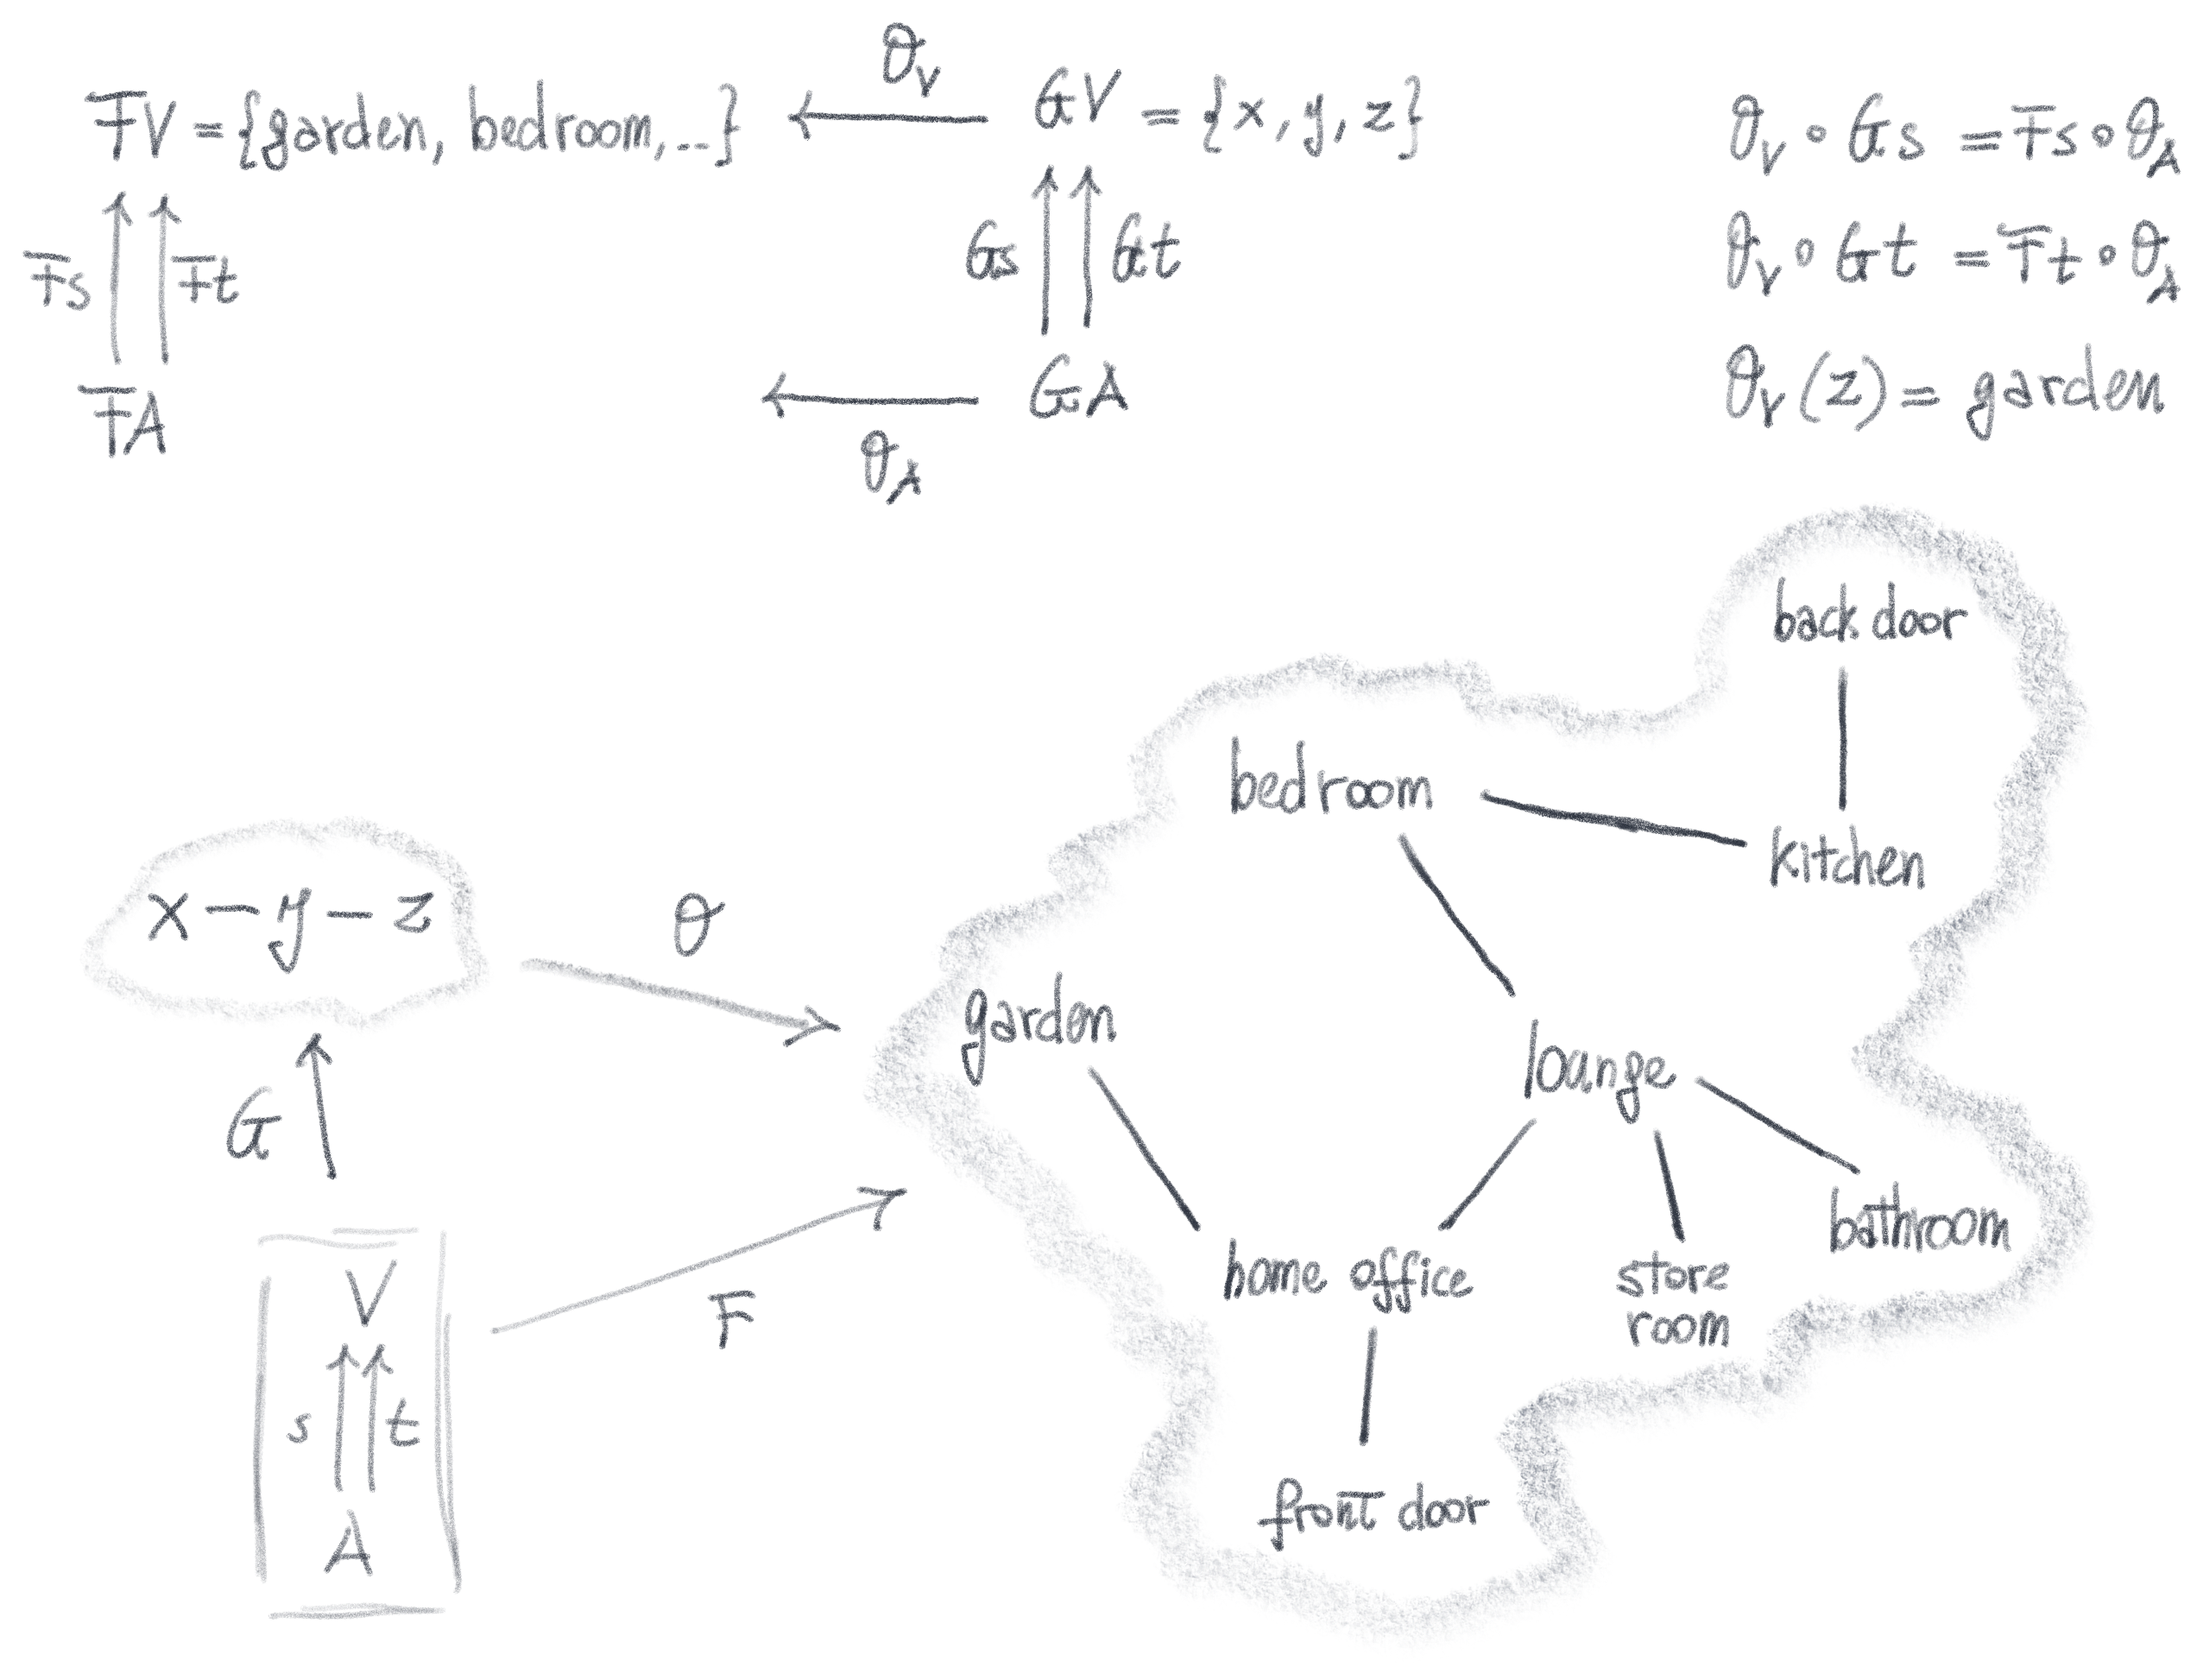
\includegraphics[height=0.8\paperheight]{./media/formal-spec_trivial-example.png}
\end{frame}
